\section{Preliminaries}
\subsection{Notations}
Let $[n]$ be a set of integers $\{1,2,\dots,n\}$ 
and let $\I(P)$ be the indicator of a predicate $P$, 
i.e., $\I(P)=1$ if $P$ is true, else $0$. 
A labeled graph is represented by a 4-tuple $G = (V, E, \mathcal{L}, l)$, 
where $V$ is a set of vertices, $E \subset V \times V$ is a set of undirected edges, 
$\mathcal{L}$ is a set of labels, and $l: V \cup E \rightarrow \mathcal{L}$ is a mapping 
that assigns a label to each vertex or edge.
We denote a subgraph isomorphism, i.e., if $g$ is a subgraph of $G$, as $G \sqsupseteq g$ 
and its negation as $G \not\sqsupseteq g$. 
Thus, a subgraph indicator $\I(G \sqsupseteq g) = 1$ if $G \sqsupseteq g$, otherwise 0.
We also denote the training set of pairs of input graph $G \in \Graph$ 
and its output responses $y \in \Y$ as
\begin{equation}
  \label{eq:train_data}
  \D = \{(G_1,y_1),(G_2,y_2),\dots,(G_N,y_N)\}.
\end{equation}
We assume that $\Graph$ is a set of all finite-size, connected, discretely-labeled, undirected graphs. 
We denote any set of graphs of size $N$ by $\Graph_N = \{G_i\mid i \in [N]\}$, 
and the set of all possible connected subgraphs 
as $\S_N = \bigcup_{G \in \Graph_N} \{g \mid G \sqsupseteq g\}$.

\begin{definition}{(subgraph isomorphism)}
	For two graphs, $G' = (V', E', \mathcal{L}', l')$ and $G = (V, E, \mathcal{L}, l)$, 
	$G'$ is subgraph isomorpic to $G$ iff there exist an injective mapping $\phi: V' \rightarrow V$, 
	s.t., (1) $\forall v \in V', l'(v) = l(\phi(v))$, 
	(2) $\forall (v_{1}, v_{2}) \in E', (\phi(v_{1}), \phi(v_{2})) \in E$ and
	(3) $l'(v_{1}, v_{2}) = l(\phi(v_{1}), \phi(v_{2}))$.
\end{definition}

\subsection{Search Space for Subgraphs}
\label{sec:subgraphMining}
In supervised learning from graphs, we represent each input graph $G_i \in
\Graph_N$ by the characteristic vector $(\I(G_i \sqsupseteq g) \mid g \in
\S) $ with a set $\S$ of relevant subgraph features. However, since $\S$ is not
explicitly available when the learning phase starts, we need to
simultaneously do searching and constructing of $\S$ during the learning process.
In order to define an efficient search space for $\S_N$, i.e., any subgraphs occurring in $\Graph_N$,
the techniques for \textit{frequent subgraph mining} \cite{Yan:2002, Nijssen:2004} are
useful. Note that any subgraph feature
$g \in \S_N$ can occur multiple times at multiple locations in a single graph,
even if $\I(G_i \sqsupseteq g) = 1$.

In the present paper, we use the search space of the gSpan algorithm \cite{Yan:2002},
which performs a depth-first search on the tree-shaped search spaces on $\S_N$,
referred to collectively as an \textit{DFS code tree}, as shown in Figure~\ref{fig:search_tree}.
Each node of the DFS code tree holds a subgraph feature $g'$ that
extends the subgraph feature $g$ at the parent node by one edge, namely, $ g' \sqsupseteq g $.

\begin{figure}[t]
  \centering
  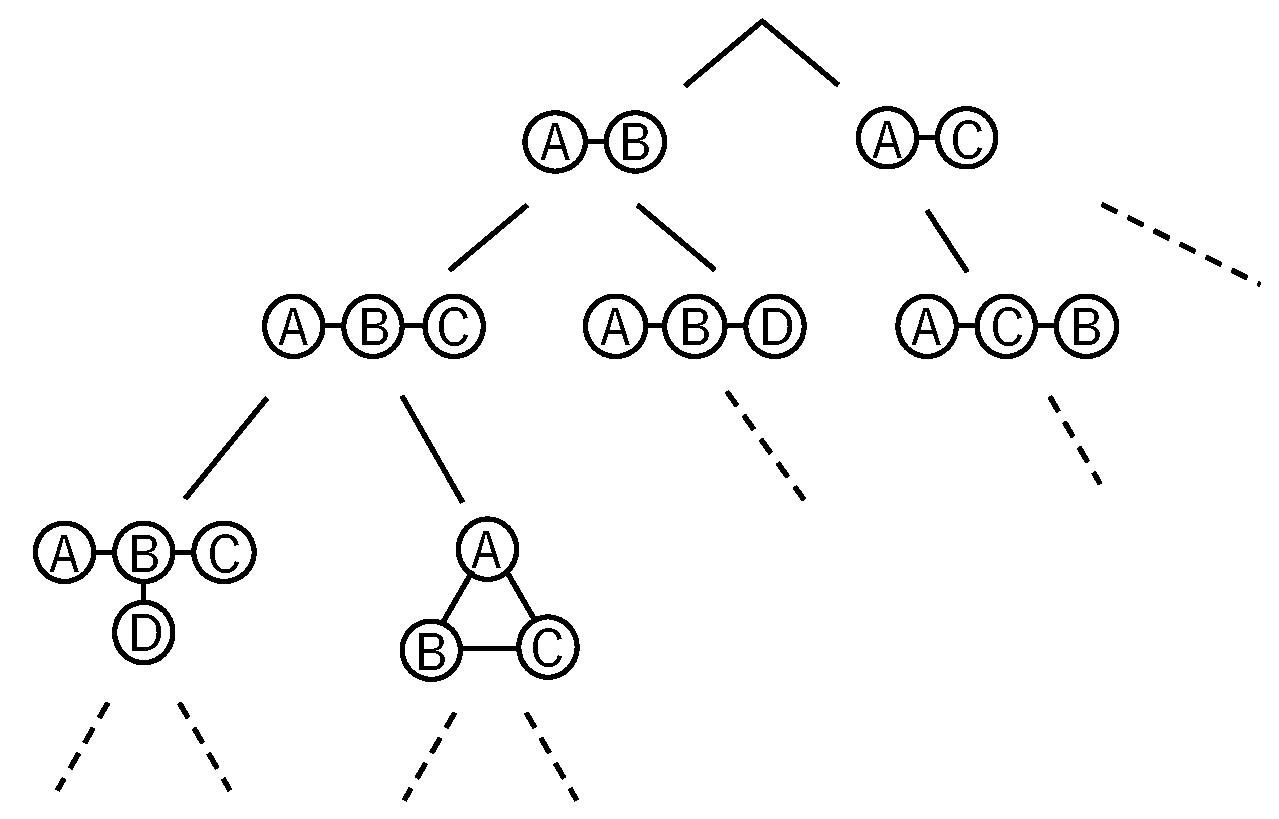
\includegraphics[width=0.5\linewidth]{img/search_tree.eps}
  \caption{DFS code tree. Search space for subgraphs that appear in the training dataset.}
  \label{fig:search_tree}
\end{figure}

The following \textit{anti-monotone} property of
subgraph isomorphism over the DFS code tree on $\S_N$ can be used to
derive the efficient search-space pruning of the gSpan algorithm:
\begin{equation}
  \label{eq:propSubgraph}
  g' \sqsupseteq g, \quad 
  G_i \not \sqsupseteq g \Rightarrow G_i \not\sqsupseteq g'. % period
\end{equation}

\subsection{Discriminative Criterion}
\label{sec:criterion}
In the previous methods, the discriminating power are calculated 
by model-based criterioa or statistical criterioa such as information gain.
In present paper, the discriminating power ($Discriminative Score: DScore$) is defined 
by the following equation.
%\begin{eqnarray}
  %\label{eq:score_C}
  %CScore(g) = \max \Big[ \sum_{n=1}^{N} y_{n} (2\I(G_{n} \sqsupseteq g) - 1), \sum_{n=1}^{N} y_{n} (2\I(G_{n} \not\sqsupseteq g) -1) \Big]
%\end{eqnarray}
%This score is the sum of the values that take +1 if the graph label prediction is correct and -1 otherwise.
%When predicting the graph labels with real values, $RegressionScore$ $(RScore)$ is used defined as (\ref{eq:score_R}).
\begin{eqnarray}
  \label{eq:score_R}
  DScore(g) &=& \tss(\D_1(g)) + \tss(\D_0(g)) \\
  \tss(\D) &=& \sum_{i \in [N]}
  (y_i - \bar{y})^2, \,\, \bar{y} = \frac{1}{N} \sum_{i \in [N]} y_i. \nonumber
\end{eqnarray}
where TSS is the total sum of squared error and
$\D_1(g) = \{ (G_i, y_i) \in \D \mid G \sqsupseteq g \} $ and
$\D_0(g) = \{ (G_i, y_i) \in \D \mid G \not\sqsupseteq g \} $.
Since this score represents an error, 
a larger value indicates lower discriminating power, 
and a smaller value indicates higher discriminating power.
This score does not depend on the learning model, 
and can be used even when the labels are discrete values.

